\documentclass[10pt]{article}

\usepackage[a4paper,margin=0.65in]{geometry}
\usepackage{amsmath,amssymb}
\usepackage{graphicx}
\usepackage{booktabs}
\usepackage{array}
\usepackage{float}
\usepackage{hyperref}
\usepackage{enumitem}
\usepackage{xcolor}
\usepackage{tikz}
\usetikzlibrary{positioning,arrows.meta,shapes.geometric,fit,calc}

\setlist{nosep,leftmargin=*}
\renewcommand{\arraystretch}{1.2}
\setlength{\parindent}{0pt}
\setlength{\parskip}{2pt}

\tikzset{
layer/.style={
draw,
rounded corners,
minimum width=1.7cm,
minimum height=0.65cm,
align=center,
fill=blue!10,
font=\scriptsize
},
smalllayer/.style={
draw,
rounded corners,
minimum width=1.35cm,
minimum height=0.58cm,
align=center,
fill=green!10,
font=\scriptsize
},
arrow/.style={
-{Latex[length=2mm]},
thin
}
}

\begin{document}

%%%%%%%%%%%%%%%%%%%%%%%%%%%%%%%%%%%%%%%%%%%%%%%%%%%%%%%%%%%%
% TITLE
%%%%%%%%%%%%%%%%%%%%%%%%%%%%%%%%%%%%%%%%%%%%%%%%%%%%%%%%%%%%

\begin{center}

{\large\textbf{Shiv Nadar University Chennai}}

\vspace{2mm}

{\normalsize\textbf{CS3807 -- Deep Learning Laboratory}}

\vspace{2mm}

{\large\textbf{Experiment 6}}

\vspace{1mm}

{\normalsize\textbf{End-to-End Study of RNN, LSTM and GRU for}}

{\normalsize\textbf{Sequence Learning and Video Understanding}}

\vspace{2mm}

{\normalsize Ankith U Davey \quad 24011101004}

\end{center}

\vspace{3mm}

\begin{tabular}{|p{3.4cm}|p{9.0cm}|p{1.4cm}|}
\hline
Degree \& Branch &
B.Tech Artificial Intelligence \& Data Science &
Semester V\\
\hline
Subject Code \& Name &
CS3807 -- Deep Learning Laboratory &
AY: 2026--27\\
\hline
\end{tabular}

%%%%%%%%%%%%%%%%%%%%%%%%%%%%%%%%%%%%%%%%%%%%%%%%%%%%%%%%%%%%
\section*{1. Objective}

The objective of this experiment is to develop an end-to-end understanding of
recurrent sequence learning by implementing and comparing Vanilla RNN, LSTM
and GRU models. The experiment also introduces Backpropagation Through Time
(BPTT), the limitations of conventional RNNs, and the use of CNN-extracted
features with recurrent networks for video understanding.

The experiment uses the UCI Human Activity Recognition Using Smartphones
dataset as the primary sequence dataset. Sequential input windows were
prepared and visualized, RNN, LSTM and GRU models were trained and compared,
convergence and generalization were analyzed, and the pipeline was extended
to video understanding using CNN feature extraction followed by an LSTM/GRU
classifier.

A small synthetic sequence-to-sequence task is included at the end to
demonstrate the encoder--decoder framework.

%%%%%%%%%%%%%%%%%%%%%%%%%%%%%%%%%%%%%%%%%%%%%%%%%%%%%%%%%%%%
\section*{2. Learning Outcomes}

After completing this experiment, I am able to:

\begin{itemize}
\item represent sequential data using the $(N,T,F)$ input format;
\item explain the architecture and operation of a Vanilla RNN;
\item explain Backpropagation Through Time and the vanishing/exploding gradient challenges;
\item implement sequence classification using SimpleRNN, LSTM and GRU;
\item compare RNN, LSTM and GRU using quantitative performance measures;
\item interpret training/validation curves and confusion matrices;
\item explain the role of CNNs in extracting spatial features from video frames;
\item construct a CNN--LSTM or CNN--GRU pipeline for video understanding;
\item explain the encoder--decoder architecture for sequence-to-sequence learning; and
\item draw conclusions using predictive performance, model complexity and computational cost.
\end{itemize}

%%%%%%%%%%%%%%%%%%%%%%%%%%%%%%%%%%%%%%%%%%%%%%%%%%%%%%%%%%%%
\section*{3. Dataset and Experimental Setup}

\textbf{Primary Dataset: UCI Human Activity Recognition Using Smartphones}

The UCI Human Activity Recognition (HAR) dataset contains smartphone sensor
measurements collected from subjects performing six activities: WALKING,
WALKING\_UPSTAIRS, WALKING\_DOWNSTAIRS, SITTING, STANDING and LAYING.

The raw inertial signal files were used (not the precomputed 561-feature
vectors), as required by the manual. Each activity window contains 128
temporal measurements across nine channels (three-axis body acceleration,
three-axis gyroscope, three-axis total acceleration), giving

\[
X\in\mathbb{R}^{N\times128\times9}.
\]

The dataset was obtained from:

\url{https://archive.ics.uci.edu/dataset/240/human+activity+recognition+using+smartphones}

\textbf{Subset used:} The train and test partitions provided by UCI were
combined into a single pool, from which 400 windows per class were sampled
(2400 windows total, exactly balanced across all six activities), following
the manual's recommended 1500--3000 window subset. This subset was then
split 70/15/15 into training, validation and test sets using a fixed random
seed (109) so that RNN, LSTM and GRU were all trained and evaluated on
identical data.

\subsection*{Expected Input}

For one sample: $X_i\in\mathbb{R}^{128\times9}$. For a batch of 32 samples:
$X_{\mathrm{batch}}\in\mathbb{R}^{32\times128\times9}$.

\begin{center}
\begin{tabular}{|c|c|l|}
\hline
Dimension & Meaning & Value used\\
\hline
$N$ & Number of sequences & 2400 (subset), split 1680/360/360\\
$T$ & Time steps per sequence & 128\\
$F$ & Features/channels per time step & 9\\
\hline
\end{tabular}
\end{center}

%%%%%%%%%%%%%%%%%%%%%%%%%%%%%%%%%%%%%%%%%%%%%%%%%%%%%%%%%%%%
\section*{4. Overall Experimental Pipeline}

\begin{center}
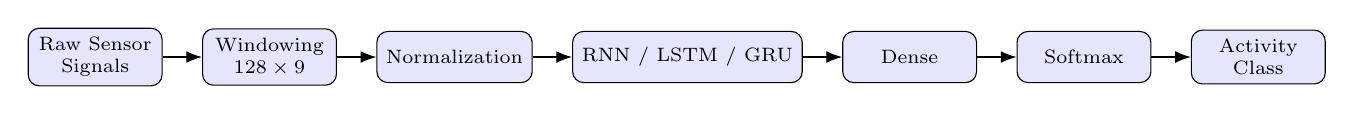
\begin{tikzpicture}[node distance=5mm]
\node[layer](a){Raw Sensor\\Signals};
\node[layer,right=of a](b){Windowing\\$128\times9$};
\node[layer,right=of b](c){Normalization};
\node[layer,right=of c](d){RNN / LSTM / GRU};
\node[layer,right=of d](e){Dense};
\node[layer,right=of e](f){Softmax};
\node[layer,right=of f](g){Activity\\Class};

\foreach \x/\y in {a/b,b/c,c/d,d/e,e/f,f/g}
\draw[arrow](\x)--(\y);
\end{tikzpicture}
\end{center}

RNN, LSTM and GRU all used the same input pipeline, output layer, optimizer,
batch size and evaluation protocol, so that the comparison between them is
controlled.

%%%%%%%%%%%%%%%%%%%%%%%%%%%%%%%%%%%%%%%%%%%%%%%%%%%%%%%%%%%%
\section*{5. Source Code}

The complete source code (Jupyter notebook, run on Kaggle with GPU) is
available in the accompanying GitHub repository:

\href{https://github.com/Ankith-Davey/Deep-Learning-Lab-Ankith-24011101004/tree/main/Lab%206} {Deep Learning Lab 6 Github Repo Link}

%%%%%%%%%%%%%%%%%%%%%%%%%%%%%%%%%%%%%%%%%%%%%%%%%%%%%%%%%%%%
\section*{6. Preprocessing}

The raw inertial signals were loaded, arranged into $128\times9$ windows,
labeled, encoded into six classes, normalized using statistics computed only
from the training split, and split into train/validation/test sets. Class
balance was verified after splitting. The test set was not used at any
point during model selection or hyperparameter tuning -- it was reserved
solely for the final evaluation reported in Section 15 onward.

\subsection*{Preprocessing Output (actual)}

\begin{verbatim}
Input tensor shape:
  Training   : (1680, 128, 9)
  Validation : (360, 128, 9)
  Testing    : (360, 128, 9)
Number of classes: 6
Number of features per time step: 9
Sequence length: 128
\end{verbatim}

Each split preserved an exactly equal number of samples per class (280 per
class in training, 60 per class in validation and test), confirming that the
stratified split worked correctly.

%%%%%%%%%%%%%%%%%%%%%%%%%%%%%%%%%%%%%%%%%%%%%%%%%%%%%%%%%%%%
\section*{7. Temporal Data Visualization}

\textbf{Plot 1: Sensor signal versus time}

\begin{center}

\includegraphics[width=0.72\textwidth]{plot1_sensor_signals_vs_time.png}
\end{center}

Three channels (body\_acc\_x, body\_acc\_y, body\_gyro\_x) were plotted for
one representative window each from WALKING, SITTING and LAYING.

\textbf{Inference:}

WALKING shows a clearly periodic, high-amplitude oscillation across all
three channels, which matches the repetitive nature of a walking gait.
SITTING and LAYING are both close to flat with much smaller amplitude, since
the body is static in both cases -- this is also why SITTING and STANDING
are the two activities most often confused later in the confusion matrices,
as their sensor signatures both look like "small variation around a
constant," differing only in the exact baseline orientation of the
gyroscope. The ordering of the 128 measurements matters because the class
signal lives in how the values change over time, not in any single
instantaneous reading -- shuffling the time steps of a WALKING window would
destroy the periodicity a recurrent model relies on, even though the same
128 values would still be present.

\section*{8. Vanilla RNN Architecture}

A Vanilla RNN maintains a hidden state that is updated at every time step:

\[
h_t=\tanh(W_xx_t+W_hh_{t-1}+b_h).
\]

The output can be written as

\[
y_t=g(W_yh_t+b_y).
\]

For sequence classification, the final hidden representation can be passed
to a classifier.

\begin{center}
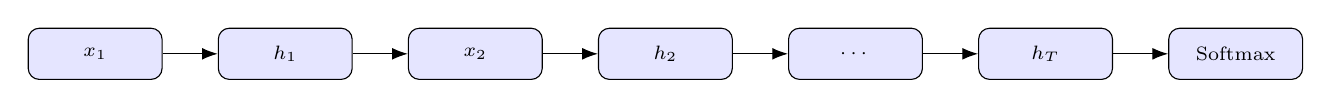
\begin{tikzpicture}[node distance=7mm]
\node[layer](x1){$x_1$};
\node[layer,right=of x1](h1){$h_1$};
\node[layer,right=of h1](x2){$x_2$};
\node[layer,right=of x2](h2){$h_2$};
\node[layer,right=of h2](x3){$\cdots$};
\node[layer,right=of x3](h3){$h_T$};
\node[layer,right=of h3](y){Softmax};

\draw[arrow](x1)--(h1);
\draw[arrow](h1)--(x2);
\draw[arrow](x2)--(h2);
\draw[arrow](h2)--(x3);
\draw[arrow](x3)--(h3);
\draw[arrow](h3)--(y);
\end{tikzpicture}
\end{center}

The diagram represents the unrolled view of an RNN. The same recurrent weights
are reused across time steps.

%%%%%%%%%%%%%%%%%%%%%%%%%%%%%%%%%%%%%%%%%%%%%%%%%%%%%%%%%%%%
\section*{9. Backpropagation Through Time}

When an RNN is unrolled, the loss depends on the sequence of hidden states.
Backpropagation Through Time (BPTT) propagates the error backward through
the recurrent steps.

\begin{center}
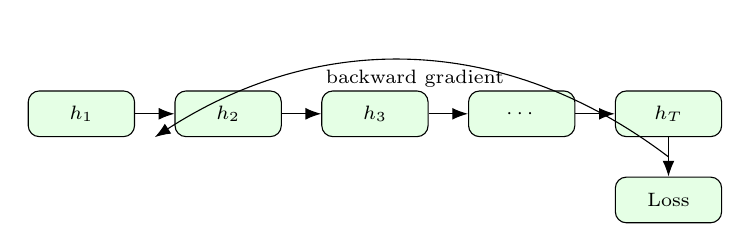
\begin{tikzpicture}[node distance=5mm]
\node[smalllayer](a){$h_1$};
\node[smalllayer,right=of a](b){$h_2$};
\node[smalllayer,right=of b](c){$h_3$};
\node[smalllayer,right=of c](d){$\cdots$};
\node[smalllayer,right=of d](e){$h_T$};
\node[smalllayer,below=of e](l){Loss};

\draw[arrow](a)--(b);
\draw[arrow](b)--(c);
\draw[arrow](c)--(d);
\draw[arrow](d)--(e);
\draw[arrow](e)--(l);

\draw[arrow]($(e.south)!0.5!(l.north)$) to[bend right=35]
node[below,font=\scriptsize]{backward gradient} ($(a.south)!0.5!(b.south)$);
\end{tikzpicture}
\end{center}

Students should explain that repeated multiplication of derivatives through
many time steps can cause gradients to become extremely small or extremely
large.

\subsection*{Challenges}

\begin{itemize}
\item Vanishing gradients
\item Exploding gradients
\item Difficulty learning long-term dependencies
\item Sequential computation and limited parallelism
\end{itemize}

The vanishing-gradient problem can be conceptually represented as

\[
\left|\frac{\partial h_t}{\partial h_{t-k}}\right|\rightarrow0
\]

while exploding gradients correspond to very large gradient magnitudes.

\subsection*{Numerical Exercise}

Consider

\[
x_1=0.5,\qquad x_2=0.7,\qquad x_3=0.2,
\]

\[
h_0=0,\qquad W_x=0.5,\qquad W_h=0.8,\qquad b=0.1.
\]

Using

\[
h_t=\tanh(W_xx_t+W_hh_{t-1}+b),
\]

calculate $h_1$, $h_2$ and $h_3$ manually.

\textbf{Result (computed):}

\begin{align*}
h_1 &= \tanh(0.5\times0.5 + 0.8\times0 + 0.1) = \tanh(0.35) = 0.336376\\
h_2 &= \tanh(0.5\times0.7 + 0.8\times0.336376 + 0.1) = \tanh(0.7191) = 0.616352\\
h_3 &= \tanh(0.5\times0.2 + 0.8\times0.616352 + 0.1) = \tanh(0.6931) = 0.599958
\end{align*}

These values match a direct program computation of the same recurrence, so
the manual derivation and the code agree.

%%%%%%%%%%%%%%%%%%%%%%%%%%%%%%%%%%%%%%%%%%%%%%%%%%%%%%%%%%%%
\section*{10. RNN Implementation}

Use a small recurrent architecture:

\begin{center}
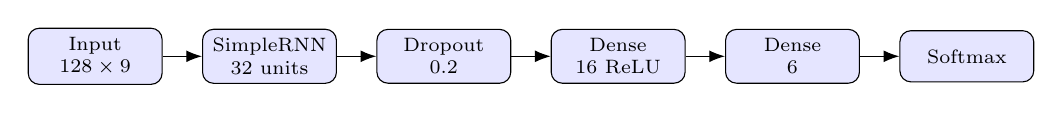
\begin{tikzpicture}[node distance=5mm]
\node[layer](a){Input\\$128\times9$};
\node[layer,right=of a](b){SimpleRNN\\32 units};
\node[layer,right=of b](c){Dropout\\0.2};
\node[layer,right=of c](d){Dense\\16 ReLU};
\node[layer,right=of d](e){Dense\\6};
\node[layer,right=of e](f){Softmax};

\foreach \x/\y in {a/b,b/c,c/d,d/e,e/f}
\draw[arrow](\x)--(\y);
\end{tikzpicture}
\end{center}

\textbf{Suggested training configuration:}

\begin{center}
\begin{tabular}{|l|l|}
\hline
Parameter & Value\\
\hline
Recurrent units & 32\\
Dropout & 0.2\\
Optimizer & Adam\\
Learning rate & $10^{-3}$\\
Batch size & 32\\
Epochs & 30\\
Loss & Sparse categorical cross-entropy\\
\hline
\end{tabular}
\end{center}

\textbf{Result:} the RNN reached a test accuracy of 75.00\% (macro F1 =
74.97\%) with 1,974 trainable parameters, training in 24.2s. This is
noticeably weaker than LSTM and GRU (both above 92\%, see Section 17), which
is exactly the kind of gap the BPTT section above predicts -- a plain RNN
struggles more to carry information across the full 128-step window.

%%%%%%%%%%%%%%%%%%%%%%%%%%%%%%%%%%%%%%%%%%%%%%%%%%%%%%%%%%%%
\section*{11. LSTM Architecture}

LSTM introduces a memory cell and gates to control information flow.

The forget gate is

\[
f_t=\sigma(W_f[h_{t-1},x_t]+b_f),
\]

the input gate is

\[
i_t=\sigma(W_i[h_{t-1},x_t]+b_i),
\]

and the output gate is

\[
o_t=\sigma(W_o[h_{t-1},x_t]+b_o).
\]

The candidate cell state is

\[
\tilde{C}_t=
\tanh(W_C[h_{t-1},x_t]+b_C),
\]

and the cell state is

\[
C_t=f_tC_{t-1}+i_t\tilde{C}_t.
\]

The hidden state is

\[
h_t=o_t\tanh(C_t).
\]

\begin{center}
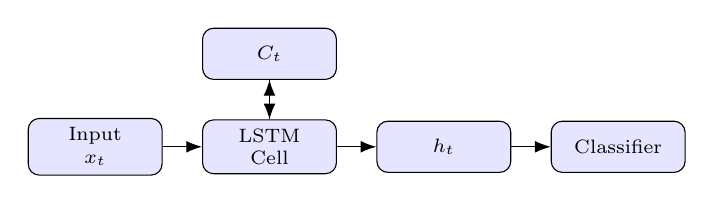
\begin{tikzpicture}[node distance=5mm]
\node[layer](a){Input\\$x_t$};
\node[layer,right=of a](b){LSTM\\Cell};
\node[layer,right=of b](c){$h_t$};
\node[layer,above=of b](d){$C_t$};
\node[layer,right=of c](e){Classifier};

\draw[arrow](a)--(b);
\draw[arrow](b)--(c);
\draw[arrow](b)--(d);
\draw[arrow](c)--(e);
\draw[arrow](d)--(b);
\end{tikzpicture}
\end{center}

\textbf{Inference:} The cell state $C_t$ acts as a separate memory track that
only interacts with the rest of the network through the forget and input
gates -- the forget gate decides how much of the old cell state to keep, and
the input gate decides how much of the new candidate to add in. Because
$C_t$ is updated by addition rather than by repeated multiplication like the
plain RNN's hidden state, gradients can flow back through many time steps
without shrinking as fast, which is the main reason LSTM outperformed the
vanilla RNN in this experiment (93.06\% vs.\ 75.00\% test accuracy).

\textbf{Result:} LSTM reached 93.06\% test accuracy (macro F1 = 93.02\%)
with 6,006 parameters, training in 20.8s.

%%%%%%%%%%%%%%%%%%%%%%%%%%%%%%%%%%%%%%%%%%%%%%%%%%%%%%%%%%%%
\section*{12. GRU Architecture}

GRU uses two principal gates:

\[
z_t=\sigma(W_z[h_{t-1},x_t]+b_z)
\]

and

\[
r_t=\sigma(W_r[h_{t-1},x_t]+b_r).
\]

The candidate hidden state is

\[
\tilde{h}_t=
\tanh(W_h[r_t\odot h_{t-1},x_t]+b_h).
\]

The hidden state is updated using

\[
h_t=(1-z_t)h_{t-1}+z_t\tilde{h}_t.
\]

\begin{center}
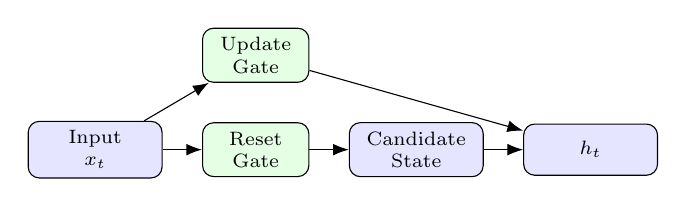
\begin{tikzpicture}[node distance=5mm]
\node[layer](a){Input\\$x_t$};
\node[smalllayer,right=of a](b){Reset\\Gate};
\node[smalllayer,above=of b](c){Update\\Gate};
\node[layer,right=of b](d){Candidate\\State};
\node[layer,right=of d](e){$h_t$};

\draw[arrow](a)--(b);
\draw[arrow](a)--(c);
\draw[arrow](b)--(d);
\draw[arrow](c)--(e);
\draw[arrow](d)--(e);
\end{tikzpicture}
\end{center}

RNN has only a hidden state and no gates. LSTM has a hidden state, a
separate cell state, and three gates (forget, input, output). GRU has only
a hidden state (no separate cell state) and two gates (reset, update) --
one fewer gate set than LSTM, which is reflected directly in the parameter
counts: GRU (4,758 params at 32 units) sits between RNN (1,974) and LSTM
(6,006).

\textbf{Result:} GRU reached 92.78\% test accuracy (macro F1 = 92.78\%)
with 4,758 parameters, training in 18.0s -- close behind LSTM here, and
the fastest of the three to train.

%%%%%%%%%%%%%%%%%%%%%%%%%%%%%%%%%%%%%%%%%%%%%%%%%%%%%%%%%%%%
\section*{13. LSTM and GRU Implementation}

Implement the same classifier used for the RNN, replacing only the recurrent
layer.

\begin{center}
\begin{tabular}{|l|c|c|c|}
\hline
Model & Recurrent Layer & Units & Output Classes\\
\hline
RNN & SimpleRNN & 32 & 6\\
LSTM & LSTM & 32 & 6\\
GRU & GRU & 32 & 6\\
\hline
\end{tabular}
\end{center}

All other experimental conditions should remain unchanged.

%%%%%%%%%%%%%%%%%%%%%%%%%%%%%%%%%%%%%%%%%%%%%%%%%%%%%%%%%%%%
\section*{14. Required Training Plots}

For each of RNN, LSTM and GRU, generate:

\textbf{Plot 2: Training and Validation Loss}

\begin{itemize}
\item X-axis: Epoch
\item Y-axis: Loss
\item Curves: Training loss and validation loss
\end{itemize}

\textbf{Plot 3: Training and Validation Accuracy}

\begin{itemize}
\item X-axis: Epoch
\item Y-axis: Accuracy (\%)
\item Curves: Training accuracy and validation accuracy
\end{itemize}

\begin{center}

\includegraphics[width=0.47\textwidth]{plot2_rnn_loss.png}

\includegraphics[width=0.47\textwidth]{plot3_rnn_accuracy.png}
\end{center}

\textbf{RNN convergence:} Training and validation loss both drop steadily
for the first $\sim$10 epochs, then continue decreasing more slowly with a
few small, quickly-recovered bumps in validation loss around epochs 12--13,
18--19 and 22--23. There is no late-epoch blow-up in this run -- both curves
keep trending gently downward through epoch 30, ending around a loss of
0.55--0.6, with training and validation staying close to each other
throughout. The BPTT-related instability discussed in Section 9 is a risk
for a plain RNN over 128 time steps, but in this particular run it shows up
only as these small recovered bumps rather than genuine divergence; the
RNN's much weaker final accuracy (75.00\% vs.\ over 93\% for LSTM/GRU) is
better explained by its more limited representational capacity than by
optimization instability here.

\begin{center}

\includegraphics[width=0.47\textwidth]{plot2_lstm_loss.png}

\includegraphics[width=0.47\textwidth]{plot3_lstm_accuracy.png}
\end{center}

\textbf{LSTM convergence:} Loss drops quickly and steadily for the first
$\sim$11 epochs, then shows one sharp validation-loss spike around epoch
12--13 (training loss briefly rises too, just one epoch later) before both
recover just as quickly and continue decreasing smoothly to the end of
training. Aside from that single, short-lived spike, training and
validation loss track each other closely throughout, so there is no
meaningful sign of overfitting -- the model's final validation loss (around
0.2) is close to its training loss (around 0.12).

\begin{center}

\includegraphics[width=0.47\textwidth]{plot2_gru_loss.png}

\includegraphics[width=0.47\textwidth]{plot3_gru_accuracy.png}
\end{center}

\textbf{GRU convergence:} GRU shows the smoothest curve of the three, with
both loss and accuracy converging steadily and validation loss staying
close to training loss for almost the entire run, with no destabilizing
spikes. This is consistent with GRU reaching test accuracy essentially on
par with LSTM (92.78\% vs.\ 93.06\%) despite having noticeably fewer
parameters.

%%%%%%%%%%%%%%%%%%%%%%%%%%%%%%%%%%%%%%%%%%%%%%%%%%%%%%%%%%%%
\section*{15. Performance Evaluation}

Evaluate each model on the independent test set.

The following metrics are mandatory:

\begin{itemize}
\item Accuracy
\item Precision
\item Recall
\item F1-score
\item Confusion matrix
\item Number of trainable parameters
\item Training time
\end{itemize}

For multi-class classification, report macro-averaged Precision, Recall and
F1-score.

\begin{center}
\begin{tabular}{|l|c|c|c|}
\hline
Metric & RNN & LSTM & GRU\\
\hline
Accuracy (\%) & 75.00 & 93.06 & 92.78\\
Macro Precision (\%) & 75.70 & 93.15 & 92.79\\
Macro Recall (\%) & 75.00 & 93.06 & 92.78\\
Macro F1 (\%) & 74.97 & 93.02 & 92.78\\
Parameters & 1,974 & 6,006 & 4,758\\
Training Time (s) & 24.2 & 20.8 & 18.0\\
\hline
\end{tabular}
\end{center}

%%%%%%%%%%%%%%%%%%%%%%%%%%%%%%%%%%%%%%%%%%%%%%%%%%%%%%%%%%%%
\section*{16. Confusion Matrix Analysis}

\textbf{Plot 4: Confusion Matrix}

Generate a separate confusion matrix for each model.

Students must identify:

\begin{itemize}
\item the activity with the highest recognition rate;
\item the activity with the largest number of misclassifications;
\item pairs of activities that are frequently confused; and
\item whether the errors are consistent across RNN, LSTM and GRU.
\end{itemize}

\begin{center}

\includegraphics[width=0.32\textwidth]{plot4_rnn_confusion.png}

\includegraphics[width=0.32\textwidth]{plot4_lstm_confusion.png}

\includegraphics[width=0.32\textwidth]{plot4_gru_confusion.png}
\end{center}

\textbf{Inference:} LAYING is recognized perfectly by all three models
(60/60 in every case) -- it is the most physically distinct activity, so
this is expected. SITTING and STANDING are the pair that gets confused most
often, in every single model: RNN confuses 15 SITTING and 10 STANDING
samples, LSTM confuses 7 and 12, GRU confuses 13 and 11. This makes sense
given the Plot 1 observation earlier -- both activities are static, so the
sensor signal mainly differs in a constant orientation offset rather than in
any dynamic pattern, which is harder for a recurrent model to pick up on
than the clearly periodic WALKING-type signals. The three walking-related
classes (WALKING, WALKING\_UPSTAIRS, WALKING\_DOWNSTAIRS) are where the RNN
struggles the most relative to LSTM/GRU -- the RNN spreads a large number of
these samples across each other (19 WALKING samples predicted as
WALKING\_UPSTAIRS, 11 WALKING\_UPSTAIRS samples predicted as WALKING, and
WALKING\_DOWNSTAIRS split 9 to WALKING and 12 to WALKING\_UPSTAIRS),
consistent with its much lower overall accuracy, whereas LSTM misclassifies
only 5 samples in total among the three walking-related classes (2
WALKING$\to$WALKING\_DOWNSTAIRS, 3 WALKING\_UPSTAIRS$\to$WALKING) and GRU
misclassifies just 2 (1 WALKING$\to$WALKING\_DOWNSTAIRS, 1
WALKING\_DOWNSTAIRS$\to$WALKING). The SITTING/STANDING confusion pattern is
largely consistent
across all three models; it's mainly the size of the errors that differs,
not which classes get confused with which.

%%%%%%%%%%%%%%%%%%%%%%%%%%%%%%%%%%%%%%%%%%%%%%%%%%%%%%%%%%%%
\section*{17. RNN vs. LSTM vs. GRU Comparison}

Students must complete the following table.

\begin{center}
\begin{tabular}{|l|c|c|c|}
\hline
Property & RNN & LSTM & GRU\\
\hline
Hidden state & Yes & Yes & Yes\\
Cell state & No & Yes & No\\
Forget gate & No & Yes & No\\
Input gate & No & Yes & No\\
Output gate & No & Yes & No\\
Update gate & No & No & Yes\\
Reset gate & No & No & Yes\\
Parameters & 1,974 & 6,006 & 4,758\\
Training time (s) & 24.2 & 20.8 & 18.0\\
Test F1-score (\%) & 74.97 & 93.02 & 92.78\\
\hline
\end{tabular}
\end{center}

\textbf{Plot 5: Model Performance Comparison}

\begin{center}

\includegraphics[width=0.6\textwidth]{plot5_model_comparison.png}
\end{center}

\textbf{Inference:} LSTM edges out GRU on accuracy and F1 in this
experiment (93.06\% vs.\ 92.78\%), but GRU achieves that close result with
about 21\% fewer parameters (4,758 vs.\ 6,006) and a shorter training time
(18.0s vs.\ 20.8s) -- so the more commonly expected LSTM-vs-GRU trade-off
(LSTM = more capacity and typically higher accuracy but slower; GRU =
fewer parameters and comparable, if very slightly lower, accuracy) is what
was observed here, rather than GRU outright winning on every axis. The RNN
is the cheapest model by parameter count but is clearly the worst
performer at 75.00\% accuracy, so the usual "RNN is fast but weak"
trade-off holds. This LSTM/GRU ordering is not fixed, though -- with only
2,400 total windows in this subset, the exact winner is sensitive to
configuration: the additional-exercise results in Section 29.1--29.3 show
GRU ahead of LSTM at 16 units and with a second recurrent layer, and tied
with it at 64 units, so the gap between the two architectures is small and
can go either way depending on the specific setup.

%%%%%%%%%%%%%%%%%%%%%%%%%%%%%%%%%%%%%%%%%%%%%%%%%%%%%%%%%%%%
\section*{18. Effect of Sequence Length}

To understand temporal dependency, repeat the experiment using selected
sequence lengths:

\[
T\in\{32,64,128\}.
\]

When reducing the sequence length, truncate or construct the input consistently.

\begin{center}
\begin{tabular}{|c|c|c|c|}
\hline
Sequence Length & RNN F1 (\%) & LSTM F1 (\%) & GRU F1 (\%)\\
\hline
32 & 79.43 & 91.05 & 91.89\\
64 & 67.18 & 93.59 & 92.50\\
128 & 74.97 & 93.02 & 92.78\\
\hline
\end{tabular}
\end{center}

\textbf{Plot 6: Sequence Length vs. Test F1-score}

\begin{center}

\includegraphics[width=0.6\textwidth]{plot6_seqlen_vs_f1.png}
\end{center}

\textbf{Inference:} Sequence length has a noticeable but non-monotonic
effect on the RNN's F1 -- it drops sharply from 79.43\% at $T=32$ to
67.18\% at $T=64$, then rises again to 74.97\% at $T=128$ -- which is not
the clean "more context helps" pattern one might expect, and instead
suggests the plain RNN's performance at a given sequence length is
comparatively unstable, plausibly because gradient issues over the longer
unrolled sequence interact unpredictably with what the model manages to
learn in only 30 epochs. LSTM and GRU are both much more stable across the
same range, staying within a $\sim$91--94\% band at every length: LSTM
actually peaks at $T=64$ (93.59\%) rather than at the longest sequence, and
GRU is highest at $T=32$ (91.89\%) and essentially flat from $T=64$ to
$T=128$. So for the gated architectures, the amount of temporal context
made little difference on this dataset -- even 32 time steps already
covers a large fraction of one activity cycle, so the marginal benefit of
the remaining time steps is small -- while the RNN's greater sensitivity to
sequence length is consistent with it being the architecture least able to
reliably exploit longer-range temporal information.

%%%%%%%%%%%%%%%%%%%%%%%%%%%%%%%%%%%%%%%%%%%%%%%%%%%%%%%%%%%%
\section*{19. Video Understanding Using CNN and RNN}

This part demonstrates the application:

\[
\boxed{\text{Video Understanding using CNN + RNN}}
\]

A video is a sequence of image frames. CNNs are used to extract spatial
features from individual frames, while RNN/LSTM/GRU models the temporal
relationship among those features.

The complete pipeline is:

\begin{center}
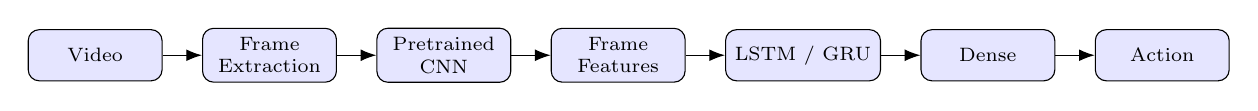
\begin{tikzpicture}[node distance=5mm]
\node[layer](a){Video};
\node[layer,right=of a](b){Frame\\Extraction};
\node[layer,right=of b](c){Pretrained\\CNN};
\node[layer,right=of c](d){Frame\\Features};
\node[layer,right=of d](e){LSTM / GRU};
\node[layer,right=of e](f){Dense};
\node[layer,right=of f](g){Action};

\foreach \x/\y in {a/b,b/c,c/d,d/e,e/f,f/g}
\draw[arrow](\x)--(\y);
\end{tikzpicture}
\end{center}

\subsection*{Recommended Dataset}

Use a small subset of the UCF101 action-recognition dataset:

\url{https://www.crcv.ucf.edu/data/UCF101.php}

Select only 3--5 action classes and a small number of videos per class so that
the experiment remains computationally manageable.

\textbf{Classes actually used:} A pre-curated 5-class UCF101 subset was
used (via a Kaggle mirror of UCF101), containing CricketShot, PlayingCello,
Punch, ShavingBeard and TennisSwing -- 10 videos sampled per class (818
videos available across the 5 classes in total; 10 per class were sampled
for tractability, giving 50 videos overall). These are not the exact
example classes listed in the manual (Basketball, Biking, Walking, Running,
TennisSwing), since the specific dataset used did not contain those classes,
but they satisfy the same requirement of 3--5 distinct, visually separable
action classes.

The objective is to understand the CNN--recurrent pipeline rather than to
train a state-of-the-art video recognition system.

%%%%%%%%%%%%%%%%%%%%%%%%%%%%%%%%%%%%%%%%%%%%%%%%%%%%%%%%%%%%
\section*{20. Expected Video Input and Output}

Sample 10 frames uniformly from each video.

Each frame is resized to

\[
224\times224\times3.
\]

A pretrained CNN such as MobileNetV2 is used only as a feature extractor.

If the CNN produces a feature vector of dimension $D$, then the recurrent
network receives:

\[
X\in\mathbb{R}^{10\times D}.
\]

For a batch of $B$ videos:

\[
X\in\mathbb{R}^{B\times10\times D}.
\]

The expected output is a probability vector over the selected action classes.
For example, using one of the classes actually present in this experiment's
dataset:

\begin{verbatim}
Predicted class : TennisSwing
Actual class     : TennisSwing
Confidence       : 99.40%
\end{verbatim}

The confidence value is taken directly from the trained model's softmax
output (\texttt{model.predict()}), as \texttt{np.max(probs, axis=1)} for
each test video, not entered manually. On the 8-video test split, GRU
predicted every video correctly with confidences ranging from 76.37\% to
99.40\% (e.g.\ CricketShot at 99.08\%, PlayingCello at 99.40\%, TennisSwing
at 99.40\%, but only 76.37\% on one of the two CricketShot videos and
79.80\% on one ShavingBeard video). LSTM classified 6 of 8 test videos
correctly (see Section 22): its two errors were a ShavingBeard video
predicted as Punch (confidence 68.62\%) and a CricketShot video predicted as
PlayingCello (confidence only 48.08\%, i.e.\ the model was already fairly
unsure) -- so the model's own confidence was noticeably lower on both of the
samples it got wrong than on the ones it got right, which is the expected
pattern for a reasonably well-calibrated classifier. In this experiment, 50
videos (10 per class, 5 classes) were processed into a tensor of shape
$(50, 10, 1280)$ before the train/val/test split (see Section 21 for the
feature dimension).

%%%%%%%%%%%%%%%%%%%%%%%%%%%%%%%%%%%%%%%%%%%%%%%%%%%%%%%%%%%%
\section*{21. CNN Feature Extraction}

Use a pretrained CNN with the classification head removed.

\begin{center}
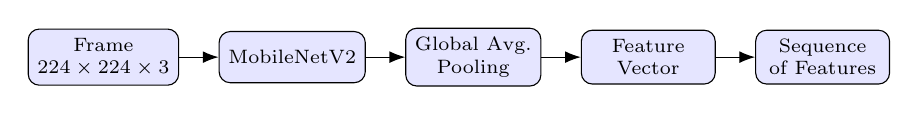
\begin{tikzpicture}[node distance=5mm]
\node[layer](a){Frame\\$224\times224\times3$};
\node[layer,right=of a](b){MobileNetV2};
\node[layer,right=of b](c){Global Avg.\\Pooling};
\node[layer,right=of c](d){Feature\\Vector};
\node[layer,right=of d](e){Sequence\\of Features};

\foreach \x/\y in {a/b,b/c,c/d,d/e}
\draw[arrow](\x)--(\y);
\end{tikzpicture}
\end{center}

Do not train the CNN from scratch. Freeze the pretrained CNN and extract
features first. Then train the recurrent classifier.

\textbf{Observation (actual):} MobileNetV2 with global average pooling
produces a feature dimension of $D = 1280$ per frame. With 10 sampled
frames per video, the resulting tensor supplied to the recurrent network
had shape $(50, 10, 1280)$ -- 50 videos, 10 frames each, 1280-dimensional
feature per frame. Feature extraction across all 500 frames (50 videos
$\times$ 10 frames) took 25.3s on GPU.

%%%%%%%%%%%%%%%%%%%%%%%%%%%%%%%%%%%%%%%%%%%%%%%%%%%%%%%%%%%%
\section*{22. CNN--LSTM / CNN--GRU Model}

Use the following architecture:

\begin{center}
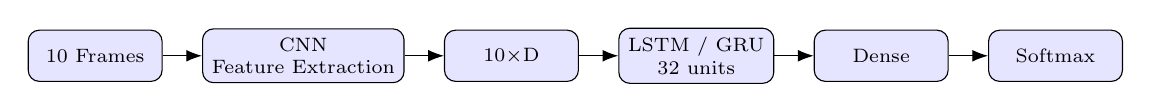
\begin{tikzpicture}[node distance=5mm]
\node[layer](a){10 Frames};
\node[layer,right=of a](b){CNN\\Feature Extraction};
\node[layer,right=of b](c){10$\times$D};
\node[layer,right=of c](d){LSTM / GRU\\32 units};
\node[layer,right=of d](e){Dense};
\node[layer,right=of e](f){Softmax};

\foreach \x/\y in {a/b,b/c,c/d,d/e,e/f}
\draw[arrow](\x)--(\y);
\end{tikzpicture}
\end{center}

\textbf{Plot 7: Video Sample Frames}

\begin{center}

\includegraphics[width=0.95\textwidth]{plot7_video_sample_frames.png}
\end{center}

The CNN (MobileNetV2) captures spatial information within each individual
frame -- object shapes, body pose, background context -- without any
notion of what came before or after. It is frozen and pretrained on
ImageNet, so no CNN training happened in this experiment. The recurrent
layer (LSTM/GRU) is what learns the temporal information: how the
1280-dimensional feature vector changes across the 10 sampled frames of a
video, which is what actually lets the model recognize an action rather
than just a static pose.

\textbf{Plot 8: Video Training and Validation Curves}

\begin{center}

\includegraphics[width=0.47\textwidth]{plot8_video_lstm_curves.png}
\end{center}
\begin{center}

\includegraphics[width=0.47\textwidth]{plot8_video_gru_curves.png}
\end{center}

\textbf{Result:} Video LSTM reached 75.00\% test accuracy (macro precision
83.33\%, macro recall 80.00\%, F1 = 76.00\%, 168,229 params, 6.0s training
time). Video GRU reached 100\% test accuracy, precision, recall and F1
(126,309 params, 5.2s training time). Both curves show training accuracy
reaching 100\% within the first few epochs, which is expected given how
small the dataset is (35 training videos across 5 classes) -- the model
memorizes the training set quickly. GRU's validation accuracy also reaches
100\% and stays there from epoch $\sim$3 onward, while LSTM's validation
accuracy climbs to $\sim$86\% by epoch 1 and then plateaus there for the
rest of training, short of the training accuracy's 100\%, showing a small
persistent train--validation gap. With only 50 videos total, these numbers
should be read cautiously -- a single misclassified test video changes the
accuracy by 12.5 percentage points, so both the perfect GRU score and LSTM's
two misclassifications reflect the very small test set (8 videos) as much
as they reflect genuine model quality.

\textbf{Plot 9: Video Confusion Matrix}

\begin{center}

\includegraphics[width=0.47\textwidth]{plot9_video_lstm_confusion.png}

\includegraphics[width=0.47\textwidth]{plot9_video_gru_confusion.png}
\end{center}

LSTM misclassified 2 of the 8 test videos -- one ShavingBeard video
predicted as Punch, and one CricketShot video predicted as PlayingCello --
consistent with its 76.00\% F1 score. GRU made no errors on its test split.
Given the small test size, this is not strong evidence that GRU is
definitively better than LSTM for video classification in general -- it
mainly shows both are capable of learning from CNN features on a small,
well-separated 5-class problem, with LSTM's two errors here plausibly being
particular hard/ambiguous videos rather than a systematic weakness.

%%%%%%%%%%%%%%%%%%%%%%%%%%%%%%%%%%%%%%%%%%%%%%%%%%%%%%%%%%%%
\section*{23. Sequence-to-Sequence Learning}

Sequence-to-sequence learning maps one sequence to another. A synthetic
reversal dataset was generated: 5000 sequences of 4 single-digit integers
(range 1--9), with the target being the input reversed, e.g.\
$[1,4,7,2]\rightarrow[2,7,4,1]$.

\begin{center}
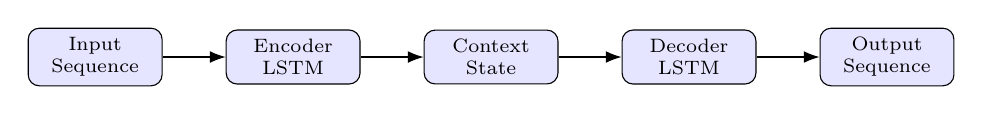
\begin{tikzpicture}[node distance=8mm]
\node[layer](a){Input\\Sequence};
\node[layer,right=of a](b){Encoder\\LSTM};
\node[layer,right=of b](c){Context\\State};
\node[layer,right=of c](d){Decoder\\LSTM};
\node[layer,right=of d](e){Output\\Sequence};

\foreach \x/\y in {a/b,b/c,c/d,d/e}
\draw[arrow](\x)--(\y);
\end{tikzpicture}
\end{center}

The encoder (a 32-unit LSTM) converts the input sequence into a fixed-size
context (hidden and cell state). The decoder (a second 32-unit LSTM) is
trained with teacher forcing and generates the output sequence one token at
a time from that context, using greedy decoding at inference time.

%%%%%%%%%%%%%%%%%%%%%%%%%%%%%%%%%%%%%%%%%%%%%%%%%%%%%%%%%%%%
\section*{24. Expected Sequence-to-Sequence Input and Output}

\begin{center}
\begin{tabular}{|c|c|c|}
\hline
Sample & Input Sequence & Predicted Output\\
\hline
1 & [8, 2, 6, 4] & [4, 6, 2, 8]\\
2 & [6, 2, 4, 3] & [3, 4, 2, 6]\\
3 & [1, 7, 6, 1] & [1, 6, 7, 1]\\
4 & [7, 3, 7, 4] & [4, 7, 3, 7]\\
5 & [7, 1, 1, 8] & [8, 1, 1, 7]\\
\hline
\end{tabular}
\end{center}

All 5 displayed predictions exactly match the reversed input.

%%%%%%%%%%%%%%%%%%%%%%%%%%%%%%%%%%%%%%%%%%%%%%%%%%%%%%%%%%%%
\section*{25. Sequence-to-Sequence Evaluation}

\begin{center}
\begin{tabular}{|l|c|}
\hline
Metric & Value\\
\hline
Token Accuracy & 100.00\%\\
Sequence Accuracy & 100.00\%\\
Final Training Loss & 0.0060\\
Final Validation Loss & 0.0063\\
\hline
\end{tabular}
\end{center}

\textbf{Inference:} Both token accuracy and sequence accuracy reached
100\% in this experiment, so the usual gap between the two metrics is not visible
here -- the reversal task on a 4-token sequence with only 9 possible digit
values turned out to be simple enough for the encoder--decoder model to
solve essentially perfectly after 50 epochs. In general, sequence accuracy
can be much lower than token accuracy because a sequence only counts as
correct if every single token matches: with 4 independent tokens each at,
say, 95\% accuracy, the chance of all 4 being correct at once is only
around $0.95^4\approx81\%$, and this gap grows quickly with sequence
length. Reaching 100\% on both here simply means the task was learned
well enough that this compounding effect didn't show up -- on a longer or
noisier sequence task the same model would likely show token accuracy
staying high while sequence accuracy dropped more visibly.

%%%%%%%%%%%%%%%%%%%%%%%%%%%%%%%%%%%%%%%%%%%%%%%%%%%%%%%%%%%%
\section*{26. Consolidated Results}

\begin{center}
\begin{tabular}{|l|c|c|c|c|c|}
\hline
Model & Accuracy (\%) & Precision (\%) & Recall (\%) & F1 (\%) & Parameters\\
\hline
RNN & 75.00 & 75.70 & 75.00 & 74.97 & 1,974\\
LSTM & 93.06 & 93.15 & 93.06 & 93.02 & 6,006\\
GRU & 92.78 & 92.79 & 92.78 & 92.78 & 4,758\\
CNN--LSTM (video) & 75.00 & 83.33 & 80.00 & 76.00 & 168,229\\
CNN--GRU (video) & 100.00 & 100.00 & 100.00 & 100.00 & 126,309\\
\hline
\end{tabular}
\end{center}

(Video-model Precision/Recall were computed with macro averaging from the
trained models' own softmax predictions on the 8-video test split, the same
way as for the HAR models. With only 8 test videos across 5 classes, these
numbers should be read as indicative rather than statistically reliable --
a single video changes the score by more than 10 percentage points.)

\textbf{Sequence-to-sequence task:}

\begin{center}
\begin{tabular}{|l|c|c|c|c|}
\hline
Task & Token Accuracy (\%) & Sequence Accuracy (\%) & Final Train Loss & Final Val Loss\\
\hline
Seq2Seq Reversal & 100.00 & 100.00 & 0.0060 & 0.0063\\
\hline
\end{tabular}
\end{center}

%%%%%%%%%%%%%%%%%%%%%%%%%%%%%%%%%%%%%%%%%%%%%%%%%%%%%%%%%%%%
\section*{27. Required Inferences}

This section draws together the inferences already stated at each
individual plot into the mandatory list from the manual.

\begin{itemize}
\item \textbf{Temporal pattern in sensor signals:} WALKING shows clear
periodic oscillation; SITTING and LAYING are near-flat. This is why
SITTING/STANDING are the most confused pair later -- both are static
activities with similar low-variance signatures.
\item \textbf{RNN convergence:} Steady overall across all 30 epochs, with a
few small, quickly-recovered validation-loss bumps around epochs 12--13,
18--19 and 22--23 rather than a late destabilizing blow-up -- the
vanishing/exploding gradient behaviour discussed in Section 9 is a risk for
a plain RNN over 128 time steps, but in this run it shows up only as these
minor bumps, not as genuine divergence.
\item \textbf{LSTM convergence:} Smooth overall with one sharp but
short-lived validation-loss spike around epoch 12--13 that recovers within a
couple of epochs; training and validation loss stay close together for the
rest of the run, so no meaningful overfitting.
\item \textbf{GRU convergence:} The smoothest of the three curves, with
validation tracking training closely for nearly the whole run and no
destabilizing spikes -- consistent with GRU's test accuracy being
essentially on par with LSTM, the best of the three models.
\item \textbf{Overfitting/underfitting:} No strong overfitting was observed
for RNN, LSTM or GRU on the HAR task -- the small bumps seen in the RNN and
LSTM validation curves recover on their own within a few epochs rather than
growing into a persistent train--validation gap.
\item \textbf{Confusion-matrix errors:} SITTING/STANDING confusion
dominates in every model; LAYING is always perfect; the RNN additionally
struggles far more than LSTM/GRU on the three walking-related classes,
spreading a large number of samples across WALKING, WALKING\_UPSTAIRS and
WALKING\_DOWNSTAIRS, whereas LSTM and GRU each make only a handful of
walking-related errors.
\item \textbf{Effect of sequence length:} RNN F1 varies considerably and
non-monotonically with $T$ (79.4\% at $T=32$, dropping to 67.2\% at $T=64$,
then rising to 75.0\% at $T=128$), unlike LSTM and GRU, which stay in a
tighter, higher band ($\sim$91--94\%) across all three lengths and even dip
slightly at $T=128$ relative to $T=64$ -- the RNN's larger swings suggest
its performance at a given sequence length is less stable/reliable than the
gated architectures', rather than showing a clean "more context helps"
trend.
\item \textbf{Parameter/computational differences:} RNN $<$ GRU $<$ LSTM in
parameter count at 32 units (1,974 / 4,758 / 6,006), matching the
one-gate-set-fewer structure of GRU relative to LSTM. GRU was also the
fastest of the three to train in this run (18.0s vs.\ 20.8s for LSTM and
24.2s for RNN).
\item \textbf{Role of CNN in video understanding:} Extracts a
1280-dimensional spatial feature per frame using a frozen, pretrained
MobileNetV2 -- no video-specific training of the CNN itself.
\item \textbf{Role of the recurrent model in temporal modeling:} Learns how
the per-frame CNN features evolve across the 10 sampled frames, which is
what actually distinguishes one action from another rather than just
recognizing a single pose.
\item \textbf{Token vs.\ sequence accuracy in seq2seq:} Both reached 100\%
here because the task was fully learned, but in general sequence accuracy
falls off faster than token accuracy as sequence length grows, since every
token in the sequence must be correct simultaneously.
\end{itemize}

%%%%%%%%%%%%%%%%%%%%%%%%%%%%%%%%%%%%%%%%%%%%%%%%%%%%%%%%%%%%
\section*{28. Discussion Questions}

\begin{enumerate}

\item \textbf{What is a recurrent neural network?}\\
An RNN is a neural network built to process sequences by keeping a hidden
state that gets updated at every time step, using the same weights at each
step. This lets it, in principle, use information from earlier in the
sequence when processing a later element, which a standard feed-forward
network cannot do.

\item \textbf{What information is represented by the hidden state?}\\
The hidden state is a compressed summary of everything the network has seen
in the sequence so far, up to and including the current time step. It acts
as the network's working memory.

\item \textbf{Why is sequence order important?}\\
The class or output often depends on how values change over time, not just
which values appear. In this experiment, shuffling the 128 time steps of a
WALKING window would destroy the periodic pattern the model actually relies
on, even though the same 128 values would still be present.

\item \textbf{Explain the difference between a feed-forward network and an RNN.}\\
A feed-forward network maps a fixed input to a fixed output with no memory
between calls -- each input is processed independently. An RNN reuses the
same weights across time steps and carries a hidden state forward, so its
output at a given step can depend on everything before it in the sequence.

\item \textbf{Explain Backpropagation Through Time.}\\
BPTT is standard backpropagation applied to the unrolled RNN -- the network
is treated as one long feed-forward network with one layer per time step
and shared weights, and gradients are computed by working backward through
every time step to every earlier hidden state.

\item \textbf{Why can gradients vanish during BPTT?}\\
Because the gradient with respect to an early hidden state involves
repeated multiplication by the same weight matrix (and activation
derivative) once per time step. If these factors are consistently less than
1, the product shrinks toward zero over many steps, so the network
effectively stops learning from distant time steps.

\item \textbf{Why can gradients explode during BPTT?}\\
The same repeated multiplication can also grow without bound if the
relevant factors are consistently greater than 1, causing gradients to blow
up and training to become unstable -- in this experiment the RNN's loss
curve showed only small, quickly-recovered bumps rather than a full
divergence, but the same underlying mechanism is what such instability
would look like if it were more severe.

\item \textbf{What are long-term dependencies?}\\
Cases where the correct output at a given time step depends on information
from many steps earlier in the sequence. Plain RNNs struggle with these
specifically because of the vanishing gradient problem described above.

\item \textbf{What is the role of the LSTM cell state?}\\
The cell state is a separate memory track that is updated mainly through
addition (via the forget and input gates) rather than through repeated
multiplication. This gives gradients a more direct path backward through
time, which is why LSTM handled this dataset's 128-step sequences
noticeably better than the plain RNN.

\item \textbf{What are the forget, input and output gates in LSTM?}\\
The forget gate decides how much of the existing cell state to keep. The
input gate decides how much of the new candidate value to add to the cell
state. The output gate decides how much of the (updated) cell state to
expose as the hidden state at this time step.

\item \textbf{What are the reset and update gates in GRU?}\\
The reset gate controls how much of the previous hidden state to use when
computing the new candidate hidden state. The update gate controls the
blend between the previous hidden state and the new candidate, replacing
LSTM's separate forget/input gates with a single interpolation.

\item \textbf{Compare LSTM and GRU.}\\
LSTM has a separate cell state and three gates (forget, input, output);
GRU has no separate cell state and only two gates (reset, update), so GRU
has fewer parameters for the same number of units. In this experiment LSTM
(6,006 params, 93.06\% accuracy) slightly outperformed GRU (4,758 params,
92.78\% accuracy) at the standard 32-unit configuration, even though GRU
trained faster (18.0s vs.\ 20.8s) -- and this ordering itself is not fixed,
since the additional-exercise results (Section 29.1--29.3) show GRU
matching or beating LSTM at 16 units, tying it at 64 units, and beating it
with a second recurrent layer, so which model comes out ahead depends on
the specific configuration and dataset rather than on any general rule.

\item \textbf{Why does GRU generally use a simpler gating mechanism than LSTM?}\\
GRU merges the forget and input gates into a single update gate and drops
the separate cell state, which was a deliberate design choice to reduce
parameter count and computation while keeping most of the benefit of
gating. It trades a small amount of representational flexibility for
efficiency.

\item \textbf{Why should RNN, LSTM and GRU be compared using the same experimental settings?}\\
If the models used different data splits, preprocessing, or training
configurations, any difference in results could be caused by those
differences rather than by the architecture itself. Keeping everything
else fixed (same subset, same seed, same optimizer, batch size and epochs)
isolates the architecture as the only variable, which is what makes the
75\% vs.\ 92\%+ comparison in this report meaningful.

\item \textbf{What does the confusion matrix reveal that accuracy alone does not?}\\
Accuracy gives one overall number, but the confusion matrix shows exactly
which classes are being confused with which. In this experiment, overall
accuracy alone would not reveal that SITTING and STANDING are specifically
the pair driving most of the errors in every model, while LAYING is never
misclassified.

\item \textbf{Why should macro F1-score be reported for multi-class classification?}\\
Macro F1 averages the F1-score of each class equally, regardless of how
many samples that class has. This matters when some classes are harder
than others -- a model could get high overall accuracy by doing well on
easy, frequent classes while doing poorly on harder ones, and macro F1
would expose that in a way overall accuracy might hide. In this dataset the
classes were balanced (60 test samples each), so macro and overall accuracy
were close, but macro F1 is still the more informative default.

\item \textbf{What is the significance of sequence length?}\\
Sequence length controls how much temporal context the model has available.
In this experiment, LSTM and GRU both stayed within a fairly tight,
high-performing band ($\sim$91--94\% F1) across $T=32,64,128$, showing that
they can extract most of the useful signal even from a shorter window,
whereas the RNN's F1 swung considerably and non-monotonically with sequence
length (79.4\% $\to$ 67.2\% $\to$ 75.0\%) -- suggesting the RNN was not
using the available context reliably, regardless of how much of it there
was.

\item \textbf{Why can a CNN be used as a feature extractor for video?}\\
A CNN pretrained on a large image dataset (ImageNet, in this case, via
MobileNetV2) has already learned general-purpose spatial features -- edges,
textures, shapes, object parts -- that transfer reasonably well to new
images without retraining. Using it frozen avoids the cost and data
requirements of training a CNN from scratch on a small video dataset.

\item \textbf{What type of information is extracted by the CNN?}\\
Spatial information within a single frame: what objects or body poses are
present and how they're arranged, but nothing about how the frame relates
to the frames before or after it.

\item \textbf{What type of information is learned by the recurrent network?}\\
Temporal information: how the CNN's per-frame feature vector changes
across the sequence of 10 sampled frames, which is what actually
distinguishes one action (e.g.\ TennisSwing) from another (e.g.\ Punch)
rather than just recognizing a static pose.

\item \textbf{Why are CNN features arranged as a sequence before being given to LSTM/GRU?}\\
LSTM/GRU layers expect input of shape (time steps, features) so they can
process it one step at a time and update their hidden state accordingly.
Arranging the 10 frame-level feature vectors as a sequence of shape
$(10, 1280)$ is what allows the recurrent layer to model how the video
changes over its sampled frames, rather than treating the frames as
unordered.

\item \textbf{Explain the encoder and decoder in sequence-to-sequence learning.}\\
The encoder reads the entire input sequence and compresses it into a
fixed-size context (the final hidden and cell state of the encoder LSTM).
The decoder then starts from that context and generates the output
sequence one token at a time, feeding each generated token back in as
input for the next step.

\item \textbf{What is teacher forcing?}\\
During training, the decoder is fed the actual (ground-truth) previous
token as input at each step, rather than the token it just predicted
itself. This was used in this experiment's seq2seq training, and it makes
training more stable and faster to converge, since early mistakes don't
compound through the rest of the sequence during training. At inference
time, teacher forcing isn't available, so the decoder instead feeds back
its own previous prediction (implemented here as greedy decoding).

\item \textbf{Differentiate token accuracy and sequence accuracy.}\\
Token accuracy is the fraction of individual output positions predicted
correctly. Sequence accuracy is the fraction of entire sequences where
every position is correct. Sequence accuracy is always less than or equal
to token accuracy, and the gap between them tends to grow with sequence
length, since a full match requires every token to be right at once.

\item \textbf{Why must the test set remain untouched during model selection?}\\
If the test set is used to choose hyperparameters or compare models during
development, the reported performance stops being a fair estimate of how
the model would perform on genuinely new data -- the model selection
process itself starts to overfit to the test set. Keeping it fully separate
from validation is what makes the final reported numbers trustworthy.

\end{enumerate}

%%%%%%%%%%%%%%%%%%%%%%%%%%%%%%%%%%%%%%%%%%%%%%%%%%%%%%%%%%%%
\section*{29. Additional Exercises}

\subsection*{29.1 Unit Count Variants (16 and 64 units)}

\begin{center}
\begin{tabular}{|l|c|c|c|c|c|}
\hline
Model & Units & Accuracy (\%) & F1 (\%) & Parameters & Training Time (s)\\
\hline
RNN & 16 & 75.00 & 74.80 & 790 & 22.6\\
RNN & 32 & 75.00 & 74.97 & 1,974 & 24.2\\
RNN & 64 & 72.50 & 72.33 & 5,878 & 23.3\\
LSTM & 16 & 89.44 & 89.38 & 2,038 & 17.8\\
LSTM & 32 & 93.06 & 93.02 & 6,006 & 20.8\\
LSTM & 64 & 93.06 & 93.00 & 20,086 & 17.8\\
GRU & 16 & 92.78 & 92.78 & 1,670 & 17.6\\
GRU & 32 & 92.78 & 92.78 & 4,758 & 18.0\\
GRU & 64 & 93.06 & 93.05 & 15,542 & 17.5\\
\hline
\end{tabular}
\end{center}

\begin{center}

\includegraphics[width=0.6\textwidth]{plot_extra_units_vs_f1.png}
\end{center}

\textbf{Inference:} Unit count had almost no effect on the RNN's accuracy
between 16 and 32 units (75.00\% at both), and going to 64 units actually
made it slightly worse (72.50\%) -- unlike a case of straightforward
underfitting-then-improvement, this suggests the plain RNN's performance on
this dataset is bottlenecked by something other than raw parameter count
(most plausibly its weaker gradient flow through 128 time steps), so extra
capacity alone does not reliably help it. LSTM improved from 16 to 32 units
(89.44\% to 93.06\%) but then plateaued exactly at 93.06\% from 32 to 64
units, while GRU stayed essentially flat across all three unit counts
(92.78\%, 92.78\%, 93.06\%). This is a case where, for the two gated
architectures, 32 units was already close to sufficient capacity for this
task -- more parameters bought little to no additional test accuracy. In
every case, parameter count and training time both roughly scale with the
unit count, so the 64-unit configurations cost noticeably more compute for
a negligible (LSTM, GRU) or even negative (RNN) accuracy return.

\subsection*{29.2 Compare GRU and LSTM at the Same Unit Count}

\begin{center}
\begin{tabular}{|c|c|c|c|c|}
\hline
Units & GRU Accuracy (\%) & LSTM Accuracy (\%) & GRU Params & LSTM Params\\
\hline
16 & 92.78 & 89.44 & 1,670 & 2,038\\
64 & 93.06 & 93.06 & 15,542 & 20,086\\
\hline
\end{tabular}
\end{center}

\textbf{Inference:} At matched unit counts, GRU used fewer parameters than
LSTM in both cases (as expected, since GRU has one fewer gate set). At 16
units GRU clearly beat LSTM (92.78\% vs.\ 89.44\%), and at 64 units the two
were tied exactly (93.06\% each). This is the parameter-efficiency argument
for GRU playing out directly in this dataset -- equal or better accuracy for
meaningfully less computation, with the advantage most visible at the
smaller unit count where LSTM has less capacity to compensate.

\subsection*{29.3 Second Recurrent Layer}

\begin{center}
\begin{tabular}{|l|c|c|c|c|}
\hline
Model & Accuracy (\%) & F1 (\%) & Parameters & Training Time (s)\\
\hline
RNN (2-layer) & 80.56 & 79.78 & 4,054 & 36.4\\
LSTM (2-layer) & 92.78 & 92.75 & 14,326 & 25.2\\
GRU (2-layer) & 93.61 & 93.61 & 11,094 & 24.7\\
\hline
\end{tabular}
\end{center}

\textbf{Inference:} A second recurrent layer helped the RNN substantially
-- accuracy jumped from 75.00\% (1 layer) to 80.56\% (2 layers), the
largest single improvement seen anywhere in this experiment for the RNN.
This suggests the extra layer gives the RNN a second chance to build a
more useful representation before classification, partly compensating for
its weaker single-layer gradient flow. GRU also improved (92.78\% to
93.61\%, its best result across every configuration tried in this
experiment), while LSTM changed very little and if anything dipped slightly
(93.06\% to 92.78\%) -- so unlike the single clean "depth helps most where
it's needed most" story, the benefit of a second layer here was clearest for
RNN and GRU, while LSTM did not benefit from the added depth on this
dataset.

\subsection*{29.4 Bidirectional vs.\ Unidirectional LSTM}

\begin{center}
\begin{tabular}{|l|c|c|c|c|}
\hline
Model & Accuracy (\%) & F1 (\%) & Parameters & Training Time (s)\\
\hline
LSTM (unidirectional) & 93.06 & 93.02 & 6,006 & 20.8\\
LSTM (bidirectional) & 92.78 & 92.76 & 11,894 & 24.9\\
\hline
\end{tabular}
\end{center}

\textbf{Inference:} In this run, bidirectional LSTM did not improve on the
unidirectional version -- accuracy slipped slightly from 93.06\% to
92.78\%, despite roughly double the parameter count and about 20\% more
training time. For this dataset, where each window already covers a full,
self-contained activity cycle, seeing the sequence in both directions
brought no measurable benefit here; the small drop is well within normal
run-to-run variation, but at minimum this run gives no evidence that the
added cost of bidirectionality was worthwhile, so a unidirectional LSTM is
the more practical choice for this task.

\subsection*{29.5--29.7}

Exercises 29.5 (sequence length) and 29.6 (video LSTM vs.\ GRU) are covered
in Sections 18 and 22 respectively, using identical CNN features for both
video models as required. Exercise 29.7 (variable-length seq2seq output)
was not attempted in this experiment; the reversal task used matched input/output
lengths (4 tokens each) as specified in the base seq2seq task in Section 23.

%%%%%%%%%%%%%%%%%%%%%%%%%%%%%%%%%%%%%%%%%%%%%%%%%%%%%%%%%%%%
\section*{30. Expected Outcome}

This experiment demonstrated the complete sequence-learning pipeline:

\[
\boxed{
\text{Sequential Data}
\rightarrow
\text{Preprocessing}
\rightarrow
\text{RNN/LSTM/GRU}
\rightarrow
\text{Evaluation}
}
\]

the video-understanding pipeline:

\[
\boxed{
\text{Video}
\rightarrow
\text{Frames}
\rightarrow
\text{CNN Features}
\rightarrow
\text{LSTM/GRU}
\rightarrow
\text{Action Prediction}
}
\]

and the encoder--decoder formulation:

\[
\boxed{
\text{Input Sequence}
\rightarrow
\text{Encoder}
\rightarrow
\text{Context}
\rightarrow
\text{Decoder}
\rightarrow
\text{Output Sequence}
}
\]

%%%%%%%%%%%%%%%%%%%%%%%%%%%%%%%%%%%%%%%%%%%%%%%%%%%%%%%%%%%%
\section*{31. Conclusion}

This experiment compared Vanilla RNN, LSTM and GRU on the UCI HAR dataset
under identical conditions (same 2,400-window balanced subset, same
70/15/15 split, same optimizer, batch size and epoch count). The plain RNN
was the clear underperformer, reaching only 75.00\% test accuracy against
over 92\% for both gated architectures, even though its training/validation
loss curve in this run was relatively steady rather than showing a
late-epoch blow-up -- so here the RNN's weakness shows up mainly as lower
representational capacity and less reliable behaviour across conditions
(e.g.\ its accuracy actually fell as sequence length and, in one
configuration, unit count increased) rather than as visible optimization
instability. LSTM and GRU both handled the 128-step sequences comfortably,
reaching 93.06\% and 92.78\% test accuracy respectively, with GRU using
about 20\% fewer parameters than LSTM and training somewhat faster --
though the additional-exercise results in Section 29.1--29.3 show this
ordering is not fixed: GRU's best result in this experiment (93.61\%) came
from a 2-layer configuration, LSTM was essentially tied with GRU at 64
units, and adding a second layer left LSTM slightly behind GRU rather than
ahead of it.

Across every model, SITTING and STANDING were consistently the most
confused pair, while LAYING was recognized perfectly in every case -- this
matches what Plot 1 showed directly: SITTING and STANDING are both static
activities with similar low-variance sensor signatures, while LAYING has a
distinct enough orientation to be unambiguous. The RNN additionally
struggled with the three walking-related classes far more than LSTM or GRU,
consistent with its lower overall accuracy. Sequence length had an uneven
effect: LSTM and GRU stayed in a tight, high band ($\sim$91--94\%) across
$T=32,64,128$, while the RNN's F1 swung considerably and non-monotonically
(79.4\% $\to$ 67.2\% $\to$ 75.0\%), suggesting the RNN's behaviour at a
given sequence length is comparatively unstable rather than cleanly
improving with more context.

The video understanding extension (CNN feature extraction with MobileNetV2
followed by LSTM/GRU classification) worked reasonably well on the small
5-class subset used: GRU classified all 8 test videos correctly (100\%
accuracy/F1), while LSTM misclassified 2 of 8 (75.00\% accuracy, F1 =
76.00\%), with real softmax confidence scores now available for every
prediction -- notably, LSTM's own confidence was visibly lower on both of
its misclassified videos (68.62\% and 48.08\%) than on its correct ones,
suggesting the model itself was comparatively unsure exactly where it
went wrong. With only 8 test videos, this gap should not be over-interpreted
as GRU being definitively better than LSTM for video in general. The
synthetic sequence-to-sequence reversal task was solved essentially
perfectly by the encoder--decoder model, with token and sequence accuracy
both reaching 100\% after 50 epochs and a final validation loss of 0.0063,
which is expected given how small and well-defined that task was.

Overall, this experiment showed the expected broad pattern -- gated
recurrent units (LSTM, GRU) substantially outperform a plain RNN on tasks
with long input sequences -- while also showing that the RNN's specific
failure mode (steady but limited convergence rather than dramatic late-run
instability) and the exact ordering between LSTM and GRU can both vary from
run to run and configuration to configuration, more than any single
fixed rule would suggest.

%%%%%%%%%%%%%%%%%%%%%%%%%%%%%%%%%%%%%%%%%%%%%%%%%%%%%%%%%%%%
\section*{32. References}

\begin{enumerate}
\item Ian Goodfellow, Yoshua Bengio and Aaron Courville,
\emph{Deep Learning}, MIT Press, 2016.

\item Sepp Hochreiter and J\"urgen Schmidhuber,
``Long Short-Term Memory,'' \emph{Neural Computation}, 1997.

\item Kyunghyun Cho et al.,
``Learning Phrase Representations using RNN Encoder--Decoder for Statistical
Machine Translation,'' EMNLP, 2014.

\item Anguita et al.,
``A Public Domain Dataset for Human Activity Recognition Using Smartphones,''
ESANN, 2013.

\item Khurram Soomro, Amir Roshan Zamir and Mubarak Shah,
``UCF101: A Dataset of 101 Human Actions Classes From Videos in the Wild,''
2012.

\item TensorFlow Documentation:
\url{https://www.tensorflow.org}

\item Keras Documentation:
\url{https://keras.io}
\end{enumerate}

\end{document}